%
% Report for the Modeling Project during our third year
% at Linköping University in the course TNM085.
%
% @author Philip Burridge, Dan Camarda,
%         Alexander Cederblad, Rasmus Haapaoja,
%         Fredrik Johnson
%

\documentclass[a4paper,12pt]{report}

% Packages
\usepackage{url}
\usepackage{amsmath}
\usepackage{mathtools}
\usepackage{lipsum}
\usepackage{listings}
\usepackage{color}
\usepackage{graphicx}
\usepackage[font=footnotesize, margin=15pt]{caption}
\usepackage{fancyhdr}

% Header customization
\setlength{\headheight}{15.2pt}
\pagestyle{fancy}
\fancyhf{}
\fancyhead[R]{\nouppercase{\leftmark}}
\cfoot{\thepage}

% Color definitions
\definecolor{mygreen}{rgb}{0,0.6,0}
\definecolor{mygray}{rgb}{0.6,0.6,0.6}
\definecolor{mymauve}{rgb}{0.58,0,0.82}

% Listing customization
\lstset{
  captionpos=b,
  numbers=left,
  frame=tb,
  showstringspaces=false,
  numbersep=15pt,
  xleftmargin=30pt,
  aboveskip=15pt,
  belowskip=15pt,
  keywordstyle=\color{blue},
  stringstyle=\color{mymauve},
  numberstyle=\color{mygray},
  rulecolor=\color{mygray}
}

% Title page customization
\title{Resolution of two dimensional collisions}
\author{Philip Burridge\\
        Dan Camarda\\
        Alexander Cederblad\\
        Rasmus Haapaoja\\
        Fredrik Johnson}
\date{\today}

%-- Start of Document
\begin{document}


%-- Title
\maketitle


%-- Abstract
\begin{abstract}
This report will cover the process of creating a physics simulation of collision impulses and their resulting frictional impulses for basic geometries. This specific simulation has been chosen due to the large use of physics simulators in today's technology. Collisions between basic geometries requires the understanding of forces acting together (gravity and friction being two examples), geometries' physical properties and their resulting interactions with one another. Due to the mathematical limitations of computers (inability to calculate continuous integration), two seperate numerical methods for integration will be covered as integration is essential for these kinds of simulations. As this simulator has been implemented in \emph{C++} and \emph{OpenGL}, the pseudo-code for the physics implementation has also been covered.
\end{abstract}


%-- Table of Contents
\tableofcontents
\addtocontents{toc}{\protect\thispagestyle{empty}}
%\listoffigures
%\listoftables
%\lstlistoflistings


%-- Introduction
\chapter{Introduction}
\setcounter{page}{1}

For this project we have chosen to simulate a general system involving collision impulse between rigid bodies in two and three dimensions. The implementation of the problem of resolving collisions includes calculating collisions between these bodies. Because of this and the fact that the focus of this project is the physical system and the numerical methods of simulation, the simplest geometries were chosen to narrow the focus. What are the simplest geometries for collision detection, you ask? Circles and spheres are the answer to your question. Since they can only collide at \emph{one} point with other convex geometries, they are the best choice to keep the focus on the simulation. Figure ~\ref{fig:snapshot} show a snapshot of this kind of simulation with circles.

\begin{figure}[!ht]
    \centering
    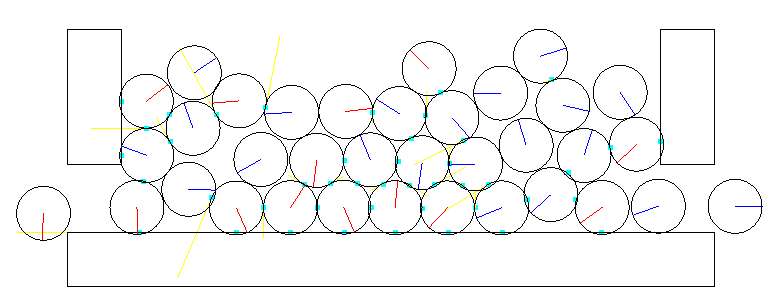
\includegraphics[width=0.8\textwidth]{figures/snapshot.png}
    \caption{A snapshop of a simulation of circles interacting with each other. The line from the origin indicates the rotation.}
    \label{fig:snapshot}
\end{figure}


%-- Physics
\chapter{Physics}

% Resolving an impulse
\section{Resolving an impulse}

To explain how to resolve an impulse\cite{gdm}, let us first think about two objects, A and B, colliding with each other, both with their own separate velocities at the collision point. Assume that we know the normal, \emph{n}, of the collision. The relative velocity $\mathbf v_{AB}$ can be calculated as shown in \ref{eq:physics:1}, where $\mathbf v_{ACP}$ and $\mathbf v_{BCP}$ is the two objects velocities at the collisions point.

\begin{equation}
\mathbf v_{AB}\cdot \mathbf n=\mathbf (\mathbf v_{ACP} - \mathbf v_{BCP})\cdot \mathbf n
\label{eq:physics:1}
\end{equation}

During a collision, an instant force i.e. an impulse will act on both objects, knocking them apart from each other. This change in the object’s relative velocity $\mathbf v'_{AB}$, as explained in \ref{eq:physics:2}, tells us that the relative velocity will be inverted proportional with the \emph{coefficient of restitution} \emph{e}. The restitution value will determine how much energy is lost during a collision. When \emph{e} is 1 no energy is lost i.e. a perfect rubber ball and when it is 0 it is a non elastic collision i.e. a clay lump hitting the floor.

\begin{equation}
\mathbf v'_{AB}\cdot \mathbf n=-e\mathbf v_{AB}\cdot \mathbf n
\label{eq:physics:2}
\end{equation}

To calculate the unknown impulse $j$ we first only take into account the object's velocities. Equations \ref{eq:physics:3} and \ref{eq:physics:4} show the change in velocity during a collision, by convension body A will add a positive velocity in the normal direction and body B will add a negative velocity.

\begin{equation}
\mathbf v'_{A}=\mathbf v_{A}+\dfrac{j}{M_{A}}\mathbf n
\label{eq:physics:3}
\end{equation}

\begin{equation}
\mathbf v'_{B}=\mathbf v_{B}-\dfrac{j}{M_{B}}\mathbf n
\label{eq:physics:4}
\end{equation}

From this we can, after some rearranging, derive a final equation for the impulse coefficient in ~\ref{eq:physics:4}.

\begin{equation}
j = \dfrac{ -(1+e) \mathbf v_{AB} \cdot \mathbf n }{
    \mathbf n \cdot \mathbf n ( \dfrac{1}{M_{A}} + \dfrac{1}{M_{A}} )}
\label{eq:physics:5}
\end{equation}

As you might have guessed by now, this equation only help resolving the \emph{linear} velocities of the rigid bodies. The following steps explains how to also account for the \emph{angular} velocities during a collision. The angular velocity is obtained as shown in \ref{eq:physics:6}, where the impulse part is positive for the object A and negative for B, just like in the case of the velocities in ~\ref{eq:physics:3} and ~\ref{eq:physics:4}. $r_{AP\perp}$ and $r_{BP\perp}$ is the perpendicular vector to the vector from the center of mass to the collision point of the two objects. $I$ is the moment of inertia of the object, determined by its geometry ~\cite{moi}.

\begin{equation}
\omega'_{A}=\omega_{A}+\dfrac{\mathbf r_{AP\perp}\cdot j\mathbf n}{I_{A}}
\label{eq:physics:6}
\end{equation}

To get the total impulse, the angular velocity is also taken into account and in the same approach as previously done the result can be derived as in \ref{eq:physics:7}. $M$ is the mass of the objects.

\begin{equation}
j = \dfrac{ -(1+e) \mathbf v_{AB} \cdot \mathbf n }{
    \mathbf n \cdot \mathbf n ( \dfrac{1}{M_{A}} + \dfrac{1}{M_{A}} )
    + \dfrac{ (\mathbf r_{AP\perp} \cdot \mathbf n)^2}{I_{A} }
    + \dfrac{ (\mathbf r_{BP\perp} \cdot \mathbf n)^2}{I_{B} } }
\label{eq:physics:7}
\end{equation}

Now that the impulse coefficient is known \ref{eq:physics:3} and \ref{eq:physics:4} can be used in the simulation. The scalar is multiplied with the normalized collision vector in both equations. This is the basic simulation; when a collision occurs, solve for the properties of the collision and then apply the impulse to the objects velocity and angular velocity.


%-- Implementation
\chapter{Implementation}

% Collision detection
\section{Collision detection}

To be able to resolve a collision impulse, an actual collision must first be registered. There is some information that we need to know about a collision to be able to resolve the collision impulse. We need to know the \emph{normal} of the collision and the \emph{collision point}. Since this is a computer simulation there will be a \emph{penetration} between the colliding object, this is also helpful to register in a collision. Figure ~\ref{fig:collision} displays a collision between two circles including this information.

\begin{figure}[!ht]
    \centering
    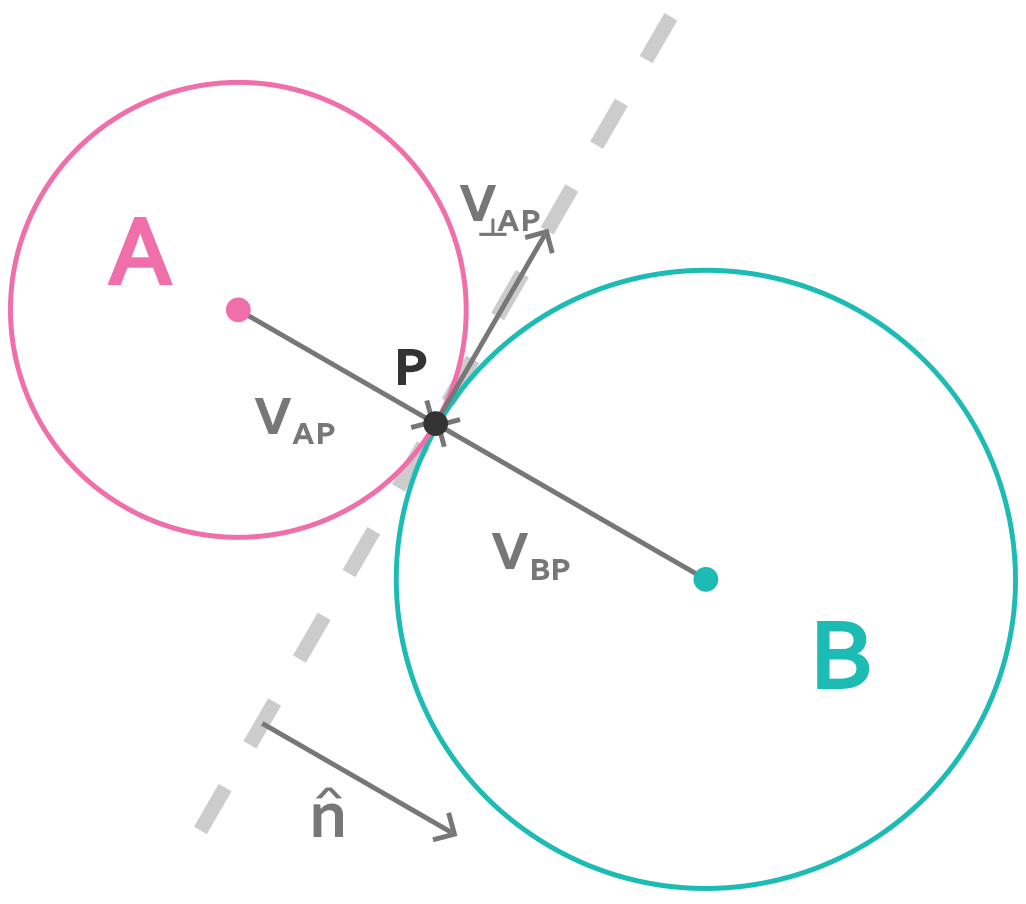
\includegraphics[width=0.6\textwidth]{figures/collision.png}
    \caption{A collision including the normal of the collision and other quantities related to the collision. The collision normal is chosen from A to B by convention.}
    \label{fig:collision}
\end{figure}

The collision detection will be different for each geometry. Circles are the simplest ones, rectangles can be handled in a few ways but the most common is the Axis-Aligned Bounding Box (AABB) method \cite{aabb}.

\subsection{Circle to Circle}

This is the simplest of all collisions to calculate. Since by convention we need to find a collision normal from object A to object B let us call the circles \emph{circle A} and \emph{circle B}. To calculate the normal the origin position of B is subtracted by the origin position A ~\ref{eq:collision:1}. It is a good idea to normalize the normal vector to ensure a proper collision impulse.

\begin{equation}
\mathbf n=\mathbf p_{B}-\mathbf p_{A}
\label{eq:collision:1}
\end{equation}

The collision position is the point on the circle's edge in the direction of the normal. That is the position of origin of circle A added with the normal vector with the same length as the radius of circle A.

\subsection{Circle to Rectangle}

To find a collision between a circle and a rectangle the closest point to collision \emph{on the rectangle} need to be calculated. This is done by clamping the circle's position value's to the rectangle edge ~\ref{eq:collision:2}.

\begin{equation}
p_{\text{closest}}=\text{clamp}( p_{\text{circle}}, p_{\text{rectangle}})
\label{eq:collision:2}
\end{equation}

The normal of the collision will then be the vector from this \emph{closest} position and the origin of the circle if by convention be have chosen the circle as body A and the circle as B. The closest collision point is illustrated in ~\ref{fig:closest}.

\begin{figure}[!ht]
    \centering
    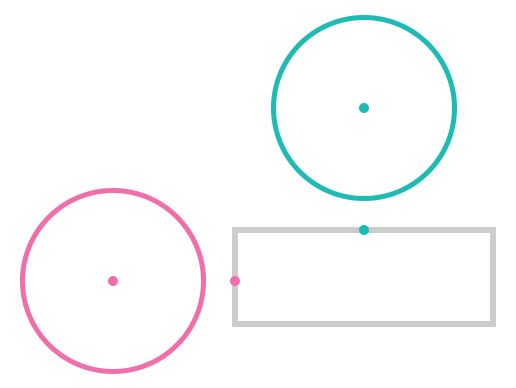
\includegraphics[width=0.4\textwidth]{figures/closest.png}
    \caption{Illustrating the closest point on a rectangle during a collision detection between a circle and a rectangle. Note that this is \emph{not a collision}.}
    \label{fig:closest}
\end{figure}


% Correcting penetration position
\section{Correcting penetration position}

As mentioned in the previous section there will be a slight penetration between the objects because of the discrete step in time between each calculation. This is not a great problem since most computers can run the simulation at a high framerate. However if the objects travel at a high enough speed they \emph{will} penetrate each other as illustrated in ~\ref{fig:penetration}, they might even skip collision if they travel past each other during a time step.

\begin{figure}[!ht]
    \centering
    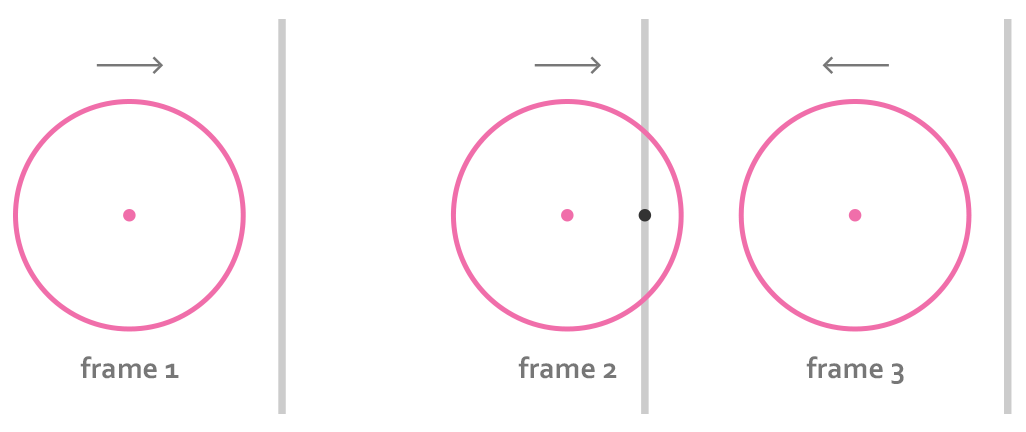
\includegraphics[width=0.6\textwidth]{figures/penetration.png}
    \caption{A collision during three time frames illustrating the penetration  where the dark dot in the second frame represents the collision position.}
    \label{fig:penetration}
\end{figure}

This effect can be handled in a few different ways, one common way is to model the penetration as a spring and separate the objects with respect to a spring coefficient and the objects' masses. In our implementation we have done a pseudo-spring solution to the problem. This effect is not clearly visable just looking at the simulation. However we have the ability to spawn objects partly penetrating another object this shows the effect very clearly. More on this in a later section (\ref{sec:opengl}) on the OpenGL implementation.


% Numerical integration
\section{Numerical integration}

\subsection{Euler method}

Since computers live in a world of zeroes and ones, we need a way to integrate numerically, the most basic and widely used approach is the \emph{Euler method}\cite{gdm}. For this type of simulation, the \emph{Euler method} is suitable for the majority of applications; however, another method will also be covered. The \emph{Euler method} \ref{eq:euler:1} works by adding the current state with its derivative multiplied by the step in time.

\begin{equation}
y_{n+1}=y_{n}+hf(t_n, y_n)
\label{eq:euler:1}
\end{equation}

In this particular simulation the method needs to be applied in two different situations. First of all to obtain the new velocities \ref{eq:euler:2} of the objects for the next frame. Which is calculated by multiplying the acceleration with the time step and then add the product to the velocity in the previous frame.

\begin{equation}
v_{t+1}=v_n+ha_n
\label{eq:euler:2}
\end{equation}

Since objects, of course, needs to be able to spin and move around in different directions for the simulation to be somewhat realistic. The positions $p$ in \ref{eq:euler:3} and orientations $\Omega$ in \ref{eq:euler:4} also needs to be updated in the scene. This is simply done by integrating the velocities $v$ and angular velocities $w$, respecivley, by multiplying with the time step.

\begin{equation}
p_{n+1}=p_n+hv_{n+1}
\label{eq:euler:3}
\end{equation}

\begin{equation}
\Omega_{n+1}=\Omega_n+h\omega_{n+1}
\label{eq:euler:4}
\end{equation}

Since this method is one of the more simplistic numerical methods, it is important to keep in mind that an error will compound with each iteration. Many times the Euler method is not good enough, the compound error increase as long as the simulation is running, as explained by \cite{gog}.

\subsection{Runge Kutta method}

As our second method we chose Runge Kutta fourth order, often referred to as classic Runge Kutta metod. This metod calculate the approximation in four increments as shown in \ref{eq:rk4:1}.

\begin{equation}
\begin{split}
\begin{aligned}
& k_{1} = f(t_{n}, x_{n}) \\
& k_{2} = f(t_{n}+\dfrac{h}{2}, x_{n}+\dfrac{h}{2}k_{1}) \\
& k_{3} = f(t_{n}+\dfrac{h}{2}, x_{n}+\dfrac{h}{2}k_{2}) \\
& k_{4} = f(t_{n}+h, x_{n}+hk_{2})
\end{aligned}
\end{split}
\label{eq:rk4:1}
\end{equation}

The step size, h, is arbitrarily chosen, to big or small will accumulate a larger error to the approximation. Like the Euler method, each step uses the previous computation to calculate a new value. To determine the next value from the present value the results from \ref{eq:rk4:1} is weighted. The two middle values are twice as important as the $k_1$ and $k_4$ as shown in \ref{eq:rk4:2}.

\begin{equation}
\begin{split}
\begin{aligned}
& dtdx = \dfrac{h}{6}(k_{1}+2k_{2}+2k_{3}+k_{4}) \\
& dtdv = \dfrac{h}{6}(k_{1}+2k_{2}+2k_{3}+k_{4})
\end{aligned}
\end{split}
\label{eq:rk4:2}
\end{equation}

The final value is the sum of the weighted values and present value \ref{eq:rk4:3}.

\begin{equation}
\begin{split}
\begin{aligned}
& x(t+1)=x(t)+dtdx\\
& v(t+1)=v(t)+dtdv
\end{aligned}
\end{split}
\label{eq:rk4:3}
\end{equation}

In our simulation Runge Kutta is applied for position, orientation, velocity and angular velocity. The improvement from Euler is showing clearly when the bodies are piled up next to each other, with zero velocity. With Euler, the balls tend to still move and never reach any steady state. The subject is futher discussed in the \emph{Discussion} chapter.


% OpenGL Implementation
\section{OpenGL implementation}
\label{sec:opengl}

The chosen method to run the simulation is \emph{OpenGL} which is a computer graphics API supported by most graphics cards. Our implementation was written in \emph{C++}. Listing \ref{lst:1} shows pseudo code for the implementation.

\begin{lstlisting}[caption={Pseudo code for the simulation loop.}, label=lst:1]
while simulation running:
    find collisions;
    apply gravitational force;
    resolve collision impulse;
    integrate resolved velocities;
    update position;
    draw objects at new position;
\end{lstlisting}


\subsection{Running the simulation}

Navigate to the folder named \emph{release} and then the OS-specific folder of your choosing click the executable file named \emph{run-simulation.*} to run the simulation. The software is not tested on any Linux distribution. These instructions are also located in the \emph{README.md} file.

\subsubsection{Requirements}
\begin{itemize}
    \item Graphics card from this century
\end{itemize}


%-- Discussion
\chapter{Discussion}

While we are quite pleased with the results of our two dimensional physics simulator, there are some definite limitations in the work. Due to the fact that our simulation only accounts for two seperate types of geometries, there is much to be desired in that respect. While the results of the simulation do mimic reality with the collisions of circles to circles and circles to rectangles, a wider array of geometries would test the capabilities of our simulator even further. This increase in collision types would certainly give us a better understanding of whether our simulator is a reliable way to imitate reality.

Another glaring problem when running the simulator is that after the majority of the collisions have occurred and the circles come to rest upon each other as well as on the rectangles, they continue to spin. Obviously, if these bodies have any type of frictional surface, they will at some point come to a rest and stop spinning. This most likely due to the fact that our friction is directly dependent on the impulse of the collisions. When two bodies are resting against one another, the collision impulse is very little (almost non-existant). This gives us a friction along the perpendicular tangent to the collision which is even less and thus, we have a frictional force which is nearly non-existant when two bodies are resting against one another. In retrospect, this is likely a case where a static friction should be implemented in addition to the dynamic friction for the two different cases.


%-- Bibliography
\bibliographystyle{vancouver}
\bibliography{report}


%-- End of Document
\end{document}
